%===================================================================%
\section*{Diagramme d'Architecture}
%===================================================================%
\begin{figure}[H]
    \centering
    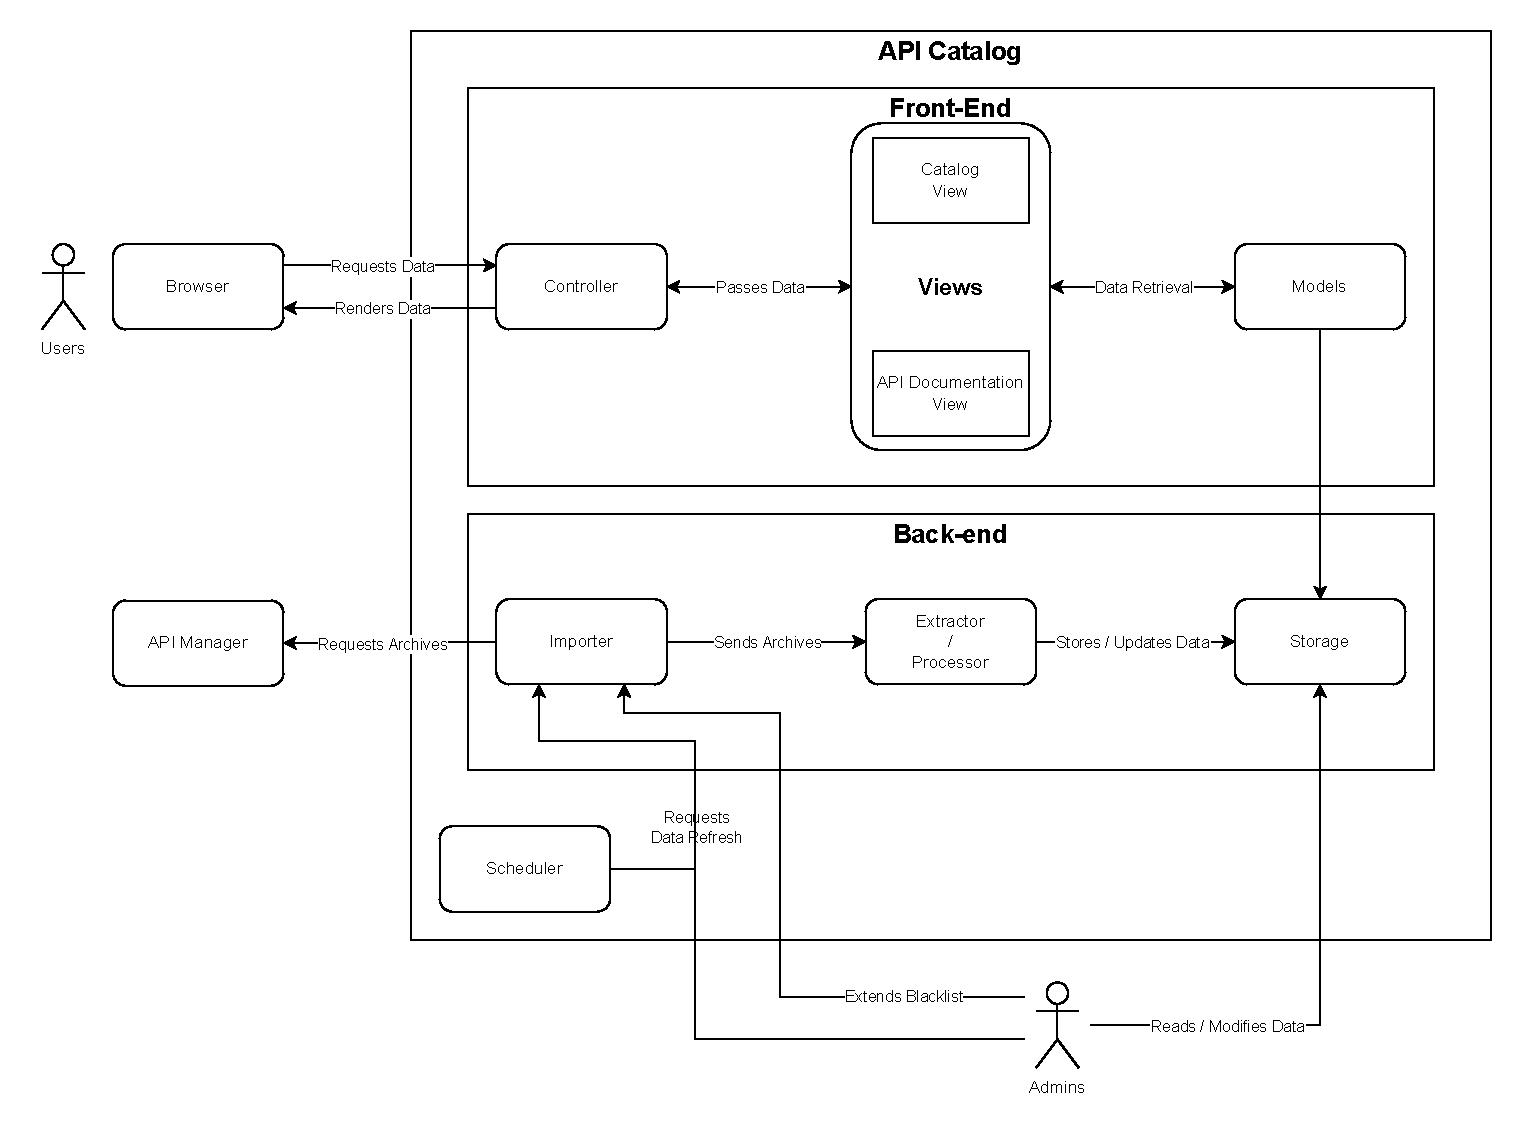
\includegraphics[width=1.\textwidth]{img/architecture_diagram.pdf}
    \caption{Diagramme d'Architecture}
\end{figure}
%%%%%%%%%%%%%%%%%%%%%%%%%%%%%%%%%%%%%%%%%%%%%%%%%%%%%%%%%%%%%%%%%%%%%
%                                                                   %
%                                                                   %
%                                                                   %
%                                                                   %
%                                                                   %
%                                                                   %
%                                                                   %
%                                                                   %
%===================================================================%
\section*{Communications entre les composants}
%===================================================================%
\begin{itemize}
    \item[$\bullet$] Front-end $\longleftrightarrow$ Back-end : volume partagé, pas de "communication" directe nécessaire

    \item[$\bullet$] Back-end :
        \begin{itemize}
        \item[$\circ$] Contient les programmes d'importation et d'extraction des données d'API
        \item[$\circ$] Tourne un serveur FastAPI qui peut servir les requêtes HTTP de l'Administrateur et du Scheduler
        \end{itemize}

    \item[$\bullet$] Scheduler :
        \begin{itemize}
        \item[$\circ$] Tourne crontab en continu
        \item[$\circ$] Crontab peut rafraîchir les données via requête HTTP vers le Back-end
        \end{itemize}

    \item[$\bullet$] Administrateur $\rightarrow$ Back-end :
        \begin{itemize}
        \item[$\circ$] Administrateur peut rafraîchir les données manuellement via requête HTTP
        \item[$\circ$] Administrateur peut consulter les données d'API via requête HTTP
        \item[$\circ$] Administrateur peut supprimer des données d'API via requête HTTP
        \end{itemize}

    \item[$\bullet$] Administrateur $\rightarrow$ Scheduler :
        \begin{itemize}
        \item[$\circ$] Administrateur peut consulter l'horaire du scheduler via requête HTTP
        \item[$\circ$] Administrateur peut changer l'horaire du scheduler via requête HTTP
        \end{itemize}
\end{itemize}
%%%%%%%%%%%%%%%%%%%%%%%%%%%%%%%%%%%%%%%%%%%%%%%%%%%%%%%%%%%%%%%%%%%%%
%                                                                   %
%                                                                   %
%                                                                   %
%                                                                   %
%                                                                   %
%                                                                   %
%                                                                   %
%                                                                   %
%===================================================================%